% A rough draft of the proof of the simple instruction reordering, given the memory model



\section{Instruction Reordering}
    Instruction reordering is a common operation in compiler optimization, essential to 
    instruction scheduling of course, but also implicit in loop invariant removal, partial redundancy
    elimination, and other optimizations that may move instructions.
    However, we saw previously how concurrent programs, under sequential consistency, may not be allowed to reorder certain events. Understanding precisely when we can safely reorder requires information on what instructions threads may be executing concurrently, which requires impractically expensive whole program analysis.
    
    \subsection{Our approach}
    Our solution to this is to construct a proof that would expose/specify the conditions under which reordering is possible given the relaxed memory semantics, while using information restricted to only the thread whose events are reordered.  We construct the proof on candidate executions of a program. To keep things simple, assume that: 
    
    \begin{enumerate}
        \item All events are tear-free
        \item No synchronize events exist
        \item No Read-Modify-Write events exist
        \item All executions of the candidate before reordering have happens-before as a strict partial order
    \end{enumerate}
    
    We first consider when consecutive events in the same agent can be reordered, followed by non-consecutive cases. The crux of the proof is to guarantee that reordering does not bring any new observable behaviors.
    
%---------------------------------------------------------------------------------------------------------------------------------------    
    \subsection{Preliminaries}
    Before we go about proving when reordering is valid, we would like to have two additional definitions which would prove useful.
    
    %Something we need to define for sake of proofs
    \begin{definition}{Consecutive pair of events (\emph{cons})}
        
        We define \emph{cons} as a function, which takes two events as input, and gives us a boolean indicating if they are consecutive pairs. Two events $e$ and $d$ are consecutive if they have an $\stck{_\textit{ao}}$ relation among them and are \emph{next to each other} in the same agent (thread), which can be defined formally as 
            \begin{align*}
                (
                e \stck{_\textit{ao}} d  \ \wedge \ 
                \nexists k \ \textit{s.t.} \ 
                e \stck{_\textit{ao}} k  \ \wedge \
                k \stck{_\textit{ao}} d 
                )
                \ \vee \
                (
                    d \stck{_\textit{ao}} e  \ \wedge \ 
                    \nexists k \ \textit{s.t.} \ 
                    d \stck{_\textit{ao}} k  \ \wedge \
                    k \stck{_\textit{ao}} e  
                )
            \end{align*}
    \end{definition}

    \begin{definition}{Direct happens-before relation (dir)}
        
        We define \emph{dir} to take an ordered pair of events $(e,d)$ such that $\reln{e}{hb}{d}$ and gives a boolean value to indicate whether this relation is \textit{direct}, i.e those relations that are not derived through transitive property of $\stck{_\textit{hb}}$.

        %Perhaps put a formal defintion here 
        
        We can infer certain relations/conditions that must hold using this function based on some information on events $e$ and $d$. 
        \begin{itemize}
            \item If $\et{e}{uo}$, then $dir(e,d) \ \Rightarrow \ cons(e,d)$
            \item If $\et{d}{uo}$, then $dir(e,d) \ \Rightarrow \ cons(e,d)$
            \item If $\et{e}{sc}\ \wedge\ e\!\in\!R$, then $dir(e,d) \ \Rightarrow \ cons(e,d)$
            \item If $\et{e}{sc}\ \wedge\ e\!\in\!W$, then $dir(e,d) \ \Rightarrow \ cons(e,d)\ \vee\ \reln{e}{sw}{d}$
            \item If $\et{d}{sc}\ \wedge\ d\!\in\!W$, then $dir(e,d) \ \Rightarrow \ cons(e,d)$
            \item If $\et{d}{sc}\ \wedge\ e\!\in\!R$, then $dir(e,d) \ \Rightarrow \ cons(e,d)\ \vee\ \reln{e}{sw}{d}$
        \end{itemize}
    \end{definition}


\subsection{Lemmas to assist our proof}    
In order to assist our proof, we define two \textit{lemmas} based on the ordering relations. 

\begin{lemma} Consider three events $e$,$d$ and $k$. \\

    If
        \[
            \cons{e}{d} \ \wedge \ \reln{e}{ao}{d} \ \wedge \
            (
                (\et{d}{uo}) \ \vee \
                (\et{d}{sc} \ \wedge \ \event{d}{W})
            )
        \]
        
    then,
        \[
            \reln{k}{hb}{d} \Longrightarrow \reln{k}{hb}{e}
        \]
      
    When we have two consecutive events \textit{e} and \textit{d} which are one after the other (i.e. $\reln{e}{ao}{d}$), we can use \textit{transitive property} of $\stck{_{hb}}$ to infer that any event \textit{k} that \textit{happens before} \textit{e}, also \textit{happens before} \textit{d}. However, is it possible to derive that the event \textit{k happens before e} using the evidence that \textit{k happens before d} ? This lemma states the condition when this is true.
    
\end{lemma}

%An alternative short proof 
\begin{proof}
    
    We will divide the proof for this into two cases, based on what event $d$ is. For both cases, we have the following to be true :
    
    \[
        cons(e,d) \ \wedge \ \reln{e}{ao}{d}
        \tag{0}
        \label{l10}
    \]

    In the first case, 
    
    \[
        \et{d}{uo} 
        \tag{1}
        \label{l11}
    \]
    
    Then for any event $k$
    \[
        dir(k,d) \Rightarrow cons(k,d)
        \qquad from \quad
        (\ref{l11})
        \tag{2}
        \label{l12}
    \]
    
    An event that satisfies the above with $d$ is $e$.
    \[
         k = e  
         \qquad from \quad
         (\ref{l10}, \ref{l12})
         \tag{3}
         \label{l13}
    \]
    
    Because $\stck{_{ao}}$ is a total order, $e$ will be the only event. This would mean that for any other $k \neq e$,
    
    \[
        \reln{k}{hb}{d} \Rightarrow \reln{k}{hb}{d}
        \qquad from \quad
        (\ref{l10}, \ref{l11}, \ref{l12}, \ref{l13}) 
    \]
    
    The following figure should explain this intuition:  
    \begin{figure}[H]
        \centering
        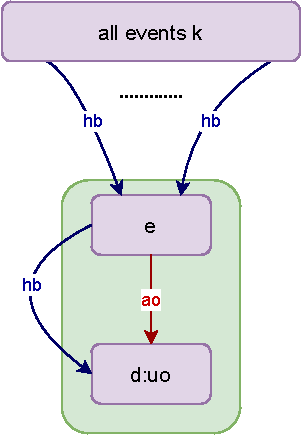
\includegraphics[scale=0.7]{InstructionReordering/Lemmas/lemma_proof1_case1.pdf}
        \caption{For the first case}
        \label{fig:my_label}
    \end{figure}
    
    In the second case,
    \[
        \et{d}{sc} \wedge d\!\in\!W
        \tag{4}
        \label{l14}
    \]
    
    Then for any event $k$
    \[
        dir(k,d) \Rightarrow cons(k,d)
        \qquad from \quad
        (\ref{l14})
        \tag{5}
        \label{l15}
    \]
    
    We once again have event $e$ satisfying the above
    \[
        k = e 
        \qquad from \quad
        (\ref{l10}, \ref{l15})
        \tag{6}
        \label{l16}
    \]
    
    Though there could be direct \textit{happens-before} relation with some event $k$ from another \textit{agent}, these are only relations satisfying $dir(d,k)$. Thus, we can once again infer that for any $k \neq e$ 
    
    \[
        \reln{k}{hb}{d} \Rightarrow \reln{k}{hb}{d}
        \qquad from \quad
        (\ref{l10}, \ref{l14}, \ref{l15}, \ref{l16})
    \]
    
    The following figure explains this intuition: 
    
    \begin{figure}[H]
        \centering
        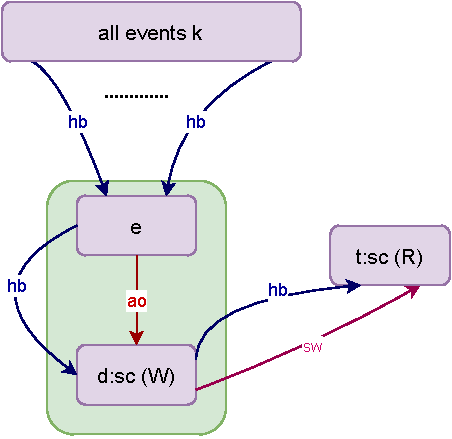
\includegraphics[scale=0.7]{InstructionReordering/Lemmas/lemma_proof1_case2.pdf}
        \caption{For the second case}
        \label{fig:my_label}
    \end{figure}
    
\end{proof}

%---------------------------------------------------------------------------------------------------------------    

%SHORTER VERSION OF PROOF WITHOUT THE ENGLISH EXPLAINATION IN THE MIDDLE. DISCUSS AND DECIDE ON WHICH FORM IS BETTER
\begin{lemma}Consider three events $e$, $d$ and $k$ \\

    If
        
        \[
            \cons{e}{d} \ \wedge \ \reln{e}{ao}{d} \ \wedge \
            (
                (\et{e}{uo}) \ \vee \
                (\et{e}{sc} \ \wedge \ \event{e}{R})
            )
        \]
        
    then,
        \[
            \reln{e}{hb}{k} \Longrightarrow \reln{d}{hb}{k}
        \]

 When we have two consecutive events \textit{e} and \textit{d} which are one after the other (i.e. $\reln{e}{ao}{d}$), we can use \textit{transitive property} of $\stck{_{hb}}$ to infer that any event \textit{k} that \textit{happens after} \textit{d}, also \textit{happens after} \textit{e}. However, is it possible to derive that the event \textit{k happens after d} using the evidence that \textit{k happens after e} ? This lemma states the condition when this is true.

\end{lemma}

%An alternative proof for this 
\begin{proof}
    
    Just like the proof for the previous lemma, we will divide the proof for this into two cases, based on what event $e$ is. Again, for both cases, we have the following to be true:
    
    \[
        cons(e,d) \ \wedge \reln{e}{ao}{d}
        \tag{0}
        \label{l20}
    \]

   In the first case,
   
   \[
        \et{e}{uo} 
        \tag{1}
        \label{l21}
   \]
   
   Then for any event k
   
   \[
        dir(e,k) \Rightarrow cons(e,k) 
        \qquad from
        \quad (\ref{l21})
        \tag{2}
        \label{l22}
   \]
   
   The event that satisfies the above with $e$ is $d$
   \[
        k = d 
        \qquad from 
        \quad (\ref{l20}, \ref{l22})
        \tag{3}
        \label{l23}
   \]
   
   Because $\stck{_{ao}}$ is a total order, $d$ would be the only such event. This would mean that for any other event $k \neq d$
   
   \[
        \reln{e}{hb}{k} \Rightarrow \reln{d}{hb}{k}
        \qquad from 
        \quad (\ref{l20}, \ref{l21}, \ref{l22}, \ref{l23})
   \]
   %Better phrase the intuition
   The following figure should explain this intuition:  
    
    \begin{figure}[H]
        \centering
        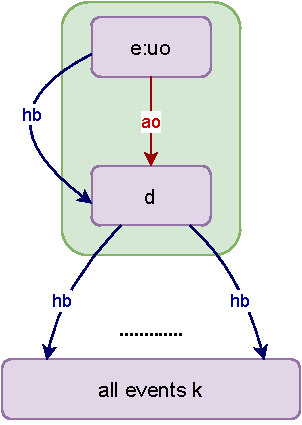
\includegraphics[scale=0.7]{InstructionReordering/Lemmas/lemma_proof2_case1.pdf}
        \caption{Caption}
        \label{fig:my_label}
    \end{figure}
    
    In the second case,
    \[
        \et{e}{sc} \wedge e\!\in\!R
        \tag{4}
        \label{l24}
    \]
    
    Then for any event $k$
    \[
        dir(e,k) \Rightarrow cons(e,k)
        \qquad from \quad
        (\ref{l24})
        \tag{5}
        \label{l25}
    \]
    
    We once again have event $d$ satisfying the above   
    \[
        k = d 
        \qquad from \quad
        (\ref{l20}, \ref{l25})
        \tag{6}
        \label{l26}
    \]
    
    Though there could be direct \textit{happens-before} relation with some event $k$ from another \textit{agent}, these are only relations satisfying $dir(k,e)$. Thus, we can once again infer that for any $k \neq d$ 
    
    \[
        \reln{e}{hb}{k} \Rightarrow \reln{d}{hb}{k}
        \qquad from \quad
        (\ref{l10}, \ref{l24},  \ref{l25}, \ref{l16})
    \]
    
    The following figure explains this intuition: 
    
    \begin{figure}[H]
        \centering
        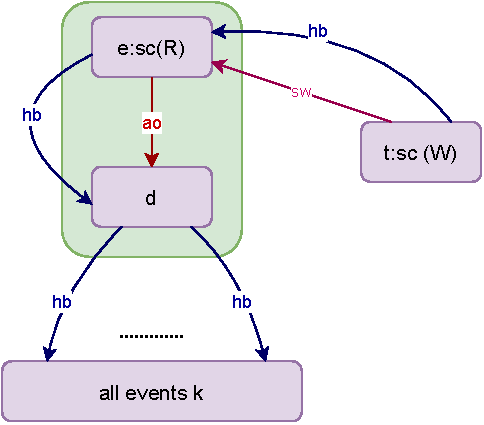
\includegraphics[scale=0.7]{InstructionReordering/Lemmas/lemma_proof2_case2.pdf}
        \caption{Caption}
        \label{fig:my_label}
    \end{figure}

\end{proof}

%------------------------------------------------------------------------------

%Uptil here, it should be constant. Henceforth, we need to start writing/ changing
%------------------------------------------------------------------------------

\subsection{Valid Reordering}
    
    We view reordering as manipulating the agent-order relation among two events. In that sense, reordering two events $e$ and $d$ with $\reln{e}{ao}{d}$ effectively flips the relation around to $\reln{d}{ao}{e}$.
%    \[
%        e \stck{_\textit{ao}} d 
%        \ \longmapsto\ 
%        d \stck{_\textit{ao}} e 
%    \]
    What implications this change has on the other ordering relations depends what events $e$ and $d$ are and would require an analysis of each Candidate Execution. We begin by first defining a reorderable pair of events. We then formulate a theorem (with proof) on the set of observable behaviors of a Candidate before and after reordering a pair of consecutive events that are reorderable. We consider reordering valid if the set of observable behaviours after reordering are a subset of the original. 
    
    \begin{definition}{Reorderable Pair (Reord)} \label{def:reord}
        We define a boolean function \emph{Reord} that takes two ordered pair of events $e$ and $d$ such that $\reln{e}{ao}{d}$ and gives a boolean value indicating if they are a reorderable pair:
         \begin{align*}
            Reord(e,d) = \\
            (
            &((\et{e}{uo} \ \wedge \ \et{d}{uo}) \ \wedge \ 
                    (   
                        (\event{e}{R} \ \wedge \ \event{d}{R}) \ \vee \ 
                        (\Re(e) \cap_\Re \Re(d) = \phi) 
                    )
            ) \\ &\vee \\
            &((\et{e}{sc} \ \wedge \ \et{d}{uo}) \ \wedge \ 
                    (
                        (\event{e}{W} \ \wedge \ (\Re(e) \cap_\Re \Re(d) = \phi)) 
                    )
            ) \\ &\vee \\
            &((\et{e}{uo} \ \wedge \ \et{d}{sc}) \ \wedge \ 
                    (
                        (\event{d}{R} \ \wedge \ (\Re(e) \cap_\Re \Re(d) = \phi)) 
                    )
            )
            )
        \end{align*}
    \end{definition}

\begin{theorem} 
    Consider a candidate $C$ of a program and its possible \textit{Candidate Executions} where $\stck{_\textit{hb}}$ is strictly partial order. Consider two events $e$ and $d$ such that $\cons{e}{d}$ is true in $C$ and  $\reln{e}{ao}{d}$. Consider another candidate $C'$ resulting after reordering $e$ and $d$. 
    Then if \emph{Reord(e,d)} is true in $C$, the set observable behaviors possible due to Candidate Executions of $C'$ is a subset of that of $C$. 
\end{theorem}

\begin{proof}

    We look at this in terms of performing an instruction reordering on a candidate execution of $C$. We would want the resulting candidate execution to preserve all the other $\stck{_{hb}}$ relations (except $\reln{e}{hb}{d}$) and that any new $\stck{_{hb}}$ relations strictly reduce possible observable behaviors. This can be summarized as addressing four main questions for any $Candidate Execution$ of $C'$:
    \begin{enumerate}
        \item Apart from $\reln{e}{hb}{d}$, do other \emph{happens-before} relations remain intact?
        \item Apart from $\reln{d}{hb}{e}$, are any new \emph{happens-before} relations established? 
        \item Are any \emph{happens-before} cycles introduced? 
        \item Do the new relations bring new \emph{observable behaviors?}
    \end{enumerate}
    
    %The first two questions ensure that existing happens-before relations are intact
    
    \subsubsection{1. Preserving \textit{happens-before} relations}
        
        If some $\stck{_{hb}}$ relations among events are missing in Candidate Executions of $C'$ as compared to that of $C$, we may introduce new observable behaviors.
        
        The relations that could be lost can be addressed by considering two disjoint sets of events in any \textit{Candidate Execution} of $C$ defined as below.
        \begin{align*}
            K_e = \{k \ | \ \reln{k}{hb}{e} \}. \\
            K_d = \{k \ | \ \reln{d}{hb}{k} \}. 
        \end{align*}
            
        Consider two events $\event{p1}{K_e}$ and $\event{p2}{K_d}$ (When $e$ is the first event or $d$ is the last event, assume dummy events that can act as $p1$ or $p2$.) belonging to the same agent as that of $e$ and $d$ such that in $C$:
        \begin{align*}
            dir(p1,e)\ \wedge\ dir(d,p2).
        \end{align*}
        
        We consider $<p1,p2>$ as a pivot pair. This pair is  \textit{valid} if 
        \begin{align*}
            \forall \ k \in K_e - \{p1\}, \ \reln{k}{hb}{p1},\ \textrm{and} \\
            \forall \ k \in K_d - \{p2\}, \ \reln{p2}{hb}{k}.
        \end{align*}
        The intuition is to $pivot$ the $\stck{_{hb}}$ relations to $p1$ and $p2$, such that after reordering $e$ and $d$, we can ``flow'' the relations back to retain all of them (due to transitivity of happens-before).
        
        By lemma 1, we have for $C$, the following condition on $e$ where $p1$ is a valid pivot
        \begin{align*}
            \et{e}{uo}\ \vee\ (\et{e}{sc}\ \wedge\ \event{e}{W}).
        \end{align*}
        
        Similarly, by lemma 2, we have for $C$, the following condition on $d$ where $p2$ is a valid pivot
        \begin{align*}
            \et{d}{uo}\ \vee\ (\et{d}{sc}\ \wedge\ \event{d}{R}).
        \end{align*}
        Table \ref{proof:table1} summarizes the cases where we have a valid pair of pivots $<p1,p2>$
        %Show a general table here 
        \begin{table}[H]
            \centering
            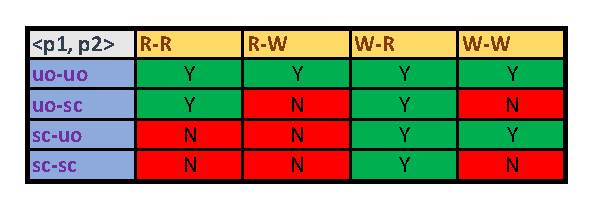
\includegraphics[scale=0.7]{Table1_Final.pdf}
            \caption{Table summarizing whether we have valid pair of pivots based on  $e$ and $d$.}
            \label{proof:table1}
        \end{table}
        \emph{Note that the relations preserved are those other than $\reln{e}{hb}{d}$. Note also that relevant happens-before relations with initialize events are always preserved. }
        
    %-------------------------------------------------------------------------------------------------------------------------------
        
    \subsubsection{2. Additional \textit{happens-before} relations}
        Among cases that have valid pair of pivots, some may introduce new $\stck{_\textit{hb}}$ relations in Candidate Executions of $C'$. As an example, for the case when $d$ is a sequentially consistent read, by lemma 1, in any Candidate Execution of $C$,
        \begin{align*}
            \reln{k}{hb}{d} \ \centernot\Rightarrow \ \reln{k}{hb}{e}.
        \end{align*}
        But in those of candidate $C'$, by transitivity, we have 
        \begin{align*}
            \reln{k}{hb}{d} \ \Rightarrow \ \reln{k}{hb}{e}.
        \end{align*}
        This is because there are sets of relations that come through $\stck{_\textit{sw}}$ relations. Table \ref{proof:table2} summarizes the cases where new relations could be introduced, assuming valid pivot pairs. 
        %Show the table here
        \begin{table}[H]
            \centering
            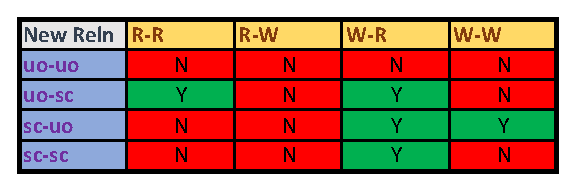
\includegraphics[scale=0.7]{Table2_Final.pdf}
            \caption{Table summarizing when new \textit{happens-before} relations could be introduced based on having valid pair of pivots.}
            \label{proof:table2}
        \end{table}
       
    %------------------------------------------------------------------------------------------------------------------------------

    \subsubsection{3. Presence of cycles?}
        Before we go into analyzing whether new relations introduce observable behaviours, we first ensure there are no $\stck{_\textit{hb}}$ cycles introduced in the process. Note that if a cycle exists in Candidate Executions of $C'$, then 
        \begin{enumerate}
            \item The relations preserved do not themselves create a cycle
            \item Additional new relations may introduce cycles
        \end{enumerate}
       
        The first part is straightforward as we assume Candidate Executions of $C$ have $\stck{_\textit{hb}}$ as a strict partial order. For the second part, we first address the case where $\reln{d}{hb}{e}$ may be part of the cycle. The other event $k$, may be either from the set $K_e$, $K_d$ or a new relation that is formed.
        
        \begin{enumerate}
            \item Event $k$ cannot belong to $K_e$ or $K_d$, as by transitive property of $\stck{_{hb}}$, a cycle would not exist. 
            \item For cases where $\reln{k}{hb}{e}$ is in the set of new relations, note that, $\reln{k}{hb}{d}$ already existed in the original Candidate Execution. On similar lines, for cases where $\reln{d}{hb}{k}$ is the set of new relations, $\reln{e}{hb}{k}$ exists. Thus, for both these cases also, a cycle with $\reln{d}{hb}{e}$  cannot exist. 
            \item For the last case where we have two new sets of relations formed, i.e $\reln{d}{hb}{k}$ and $\reln{k}{hb}{e}$, we could have a case where $k$ is a common event for both sets. By lemma 1, we also have $\reln{k}{hb}{d}$ and by lemma 2, $\reln{e}{hb}{k}$. Thus, we have a cycle. 
        \end{enumerate}
        
        For the case when $\reln{d}{hb}{e}$ may not be part of the cycle, consider the first scenario where the new set of relations are of the form $\reln{k}{hb}{e}$. Suppose a cycle exists with another event $k'$, then
        \begin{align*}
            \reln{k}{hb}{e} \ \wedge \ \reln{e}{hb}{k'} \ \wedge \ \reln{k'}{hb}{k}.
        \end{align*}
        By lemma 1, we also have $\reln{k}{hb}{d}$ and by transitivity we also have $\reln{d}{hb}{k'}$. So, the following is also a cycle
        \begin{align*}
            \reln{k}{hb}{d} \ \wedge \ \reln{d}{hb}{k'} \ \wedge \ \reln{k'}{hb}{k}.
        \end{align*}
        But these relations already existed in the original Candidate Execution, which implies a cycle existed in Candidate Execution of $C$. Thus, by contradiction, a cycle cannot exist. In similar lines we can show for the set $\reln{d}{hb}{k}$ that there cannot be any cycles. 
    
    %---------------------------------------------------------------------------------------------------------------------------------  

    \subsubsection{4. Do new relations introduce new observable behaviours}
        In any candidate execution, reordering events $e$ and $d$ eliminates the relation $\reln{e}{hb}{d}$ and introduces the new relation $\reln{d}{hb}{e}$.  New behaviours created by the latter directly, if any, are 
        of course intentional (and should normally be avoided by ensuring $e$ and $d$ are independent), but we need to ensure that this does not also result in new behaviours indirectly.

        On observing the role of the axioms on this relation, notice that if both $e$ and $d$ are read events then the range does not matter. For all other cases, if events $e$ and $d$ have overlapping ranges, one could introduce a new observable behavior after reordering them (a simple use of Coherent Reads / Sequentially Consistent Atomics).        
        Any other new relations that are introduced can be divided into 4 cases, in terms of our events $e$ and $d$ and the new relation with some event $k$:
        \begin{tasks}(2)
            \task  $\et{e}{uo} \ \wedge \ \event{e}{R} \ \wedge \ \reln{k}{hb}{e}$.
            \task  $\et{e}{uo} \ \wedge \  \event{e}{W} \ \wedge \ \reln{k}{hb}{e}$.
            \task  $\et{d}{uo} \ \wedge \  \event{d}{R} \ \wedge \ \reln{d}{hb}{k}$.
            \task  $\et{d}{uo} \ \wedge \ \event{d}{W} \ \wedge \ \reln{d}{hb}{k}$.
        \end{tasks}
        In each of the above cases, note that we need to only consider cases where their ranges are overlapping/equal.
        
        %Addressing the first case. 
        Figure~\ref{fig:subcases} shows a breakdown of sub-cases for the first case (a), varying based
        on the nature of event $k$.
        %Show all cases here for different k
        \begin{figure}
            \centering
            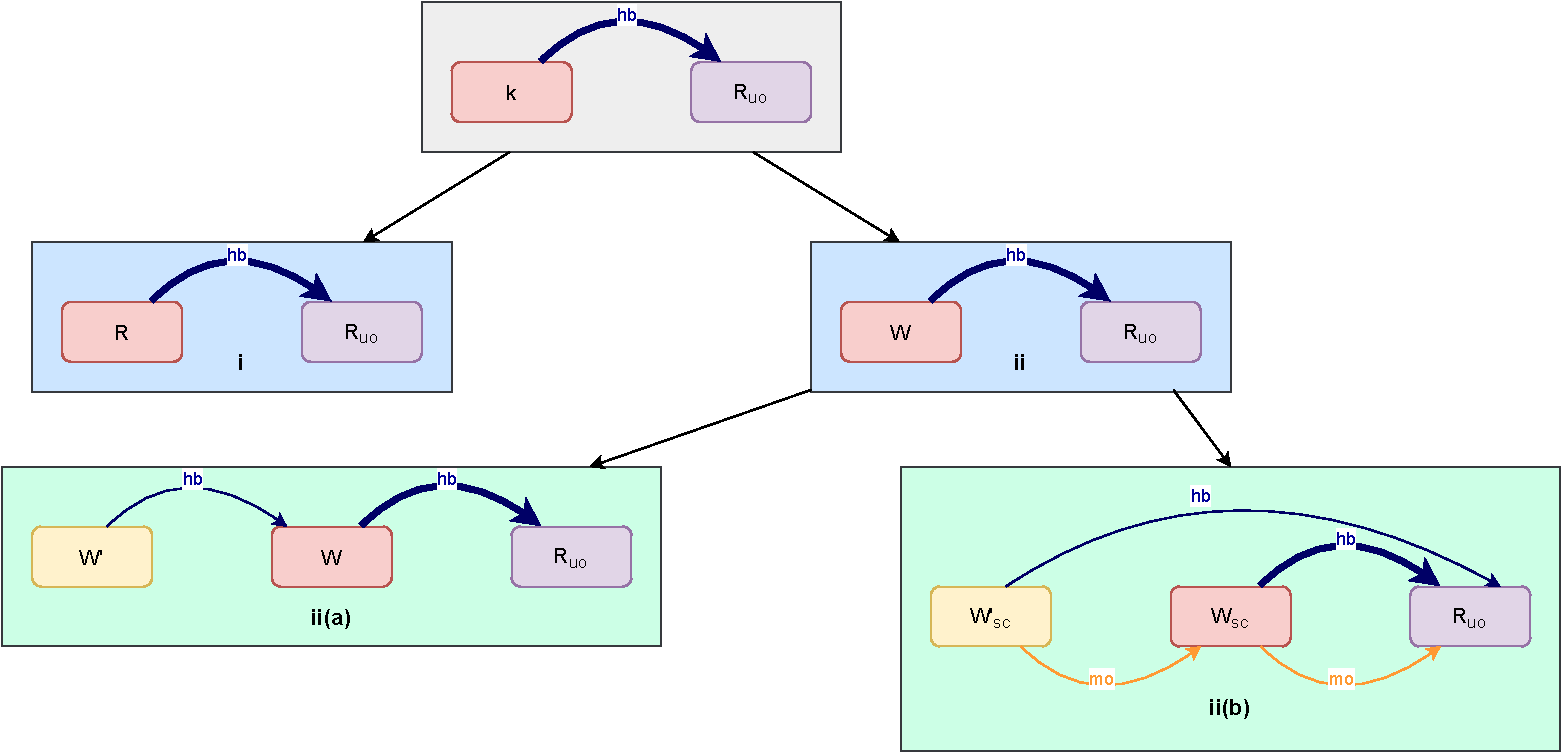
\includegraphics[width=\textwidth]{Q3_(b)Case1.pdf}
            \caption{The role of the axioms on introducing a new relation between an unordered read (purple box) and a preceding (by \textit{hb}) event $k$ (red box), varying based on whether $k$ is a read, write, or sequentially consistent write.}
            \label{fig:subcases}
        \end{figure}
        \
        %Might have to elaborate this more
        \begin{enumerate}
            \item For (i), when $k$ is a read, none of the rules have any implications on observable behaviors.
            \item For (ii), when $k$ is a write, the rule of coherent reads (ii(a)) or sequentially consistent atomics (ii(b)) could restrict the read ($e$) from reading overlapping ranges of $W'$ with $W$.
        \end{enumerate}
        
        The above case analysis shows us that the new relation could 'trigger' the consistency rules, only to restrict possible reads-from relations, thus restricting possible observable behaviors. 
       
        Similarly, for other cases, the new relations could also 'trigger' the consistency rules, but again, only  \emph{restricting} $\stck{_\textit{rf}}$ relations. 

        Table \ref{proof:table3} summarizes the valid cases where, we have a pair of valid pivots, where new relations do not introduce any $\stck{_\textit{hb}}$ cycles and may only restrict possible observable behaviors. 
        %Show the table here
        \begin{table}[H]
            \centering
            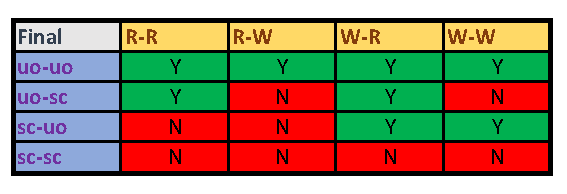
\includegraphics[scale=0.7]{Table4_Final.pdf}
            \caption{The final table summarizing the valid cases where observable behaviors will only be a subset after reordering.}
            \label{proof:table3}
        \end{table}
    
        The table above, precisely is the definition of a reorderable pair (Def.~\ref{def:reord}). \qed
                
        \vspace{1mm}Note that in the above we did not consider the $\stck{_\textit{mo}}$ relation, as preserving $\stck{_\textit{hb}}$ relations naturally preserves all the $\stck{_\textit{mo}}$ relations that must hold.
\end{proof}

    The following corollary helps us define when instruction reordering among non-consecutive events is possible.
  
%--------------------------------------------------------------------------------------------------------------------------------------

\begin{corollary}
    Consider a Candidate C of a program and its Candidate Executions which are valid. Consider two events $e$ and $d$ where $\reln{e}{ao}{d}$, but $\neg \cons{e}{d}$. Consider another Candidate C' resulting after reordering $e$ and $d$ in C. Then, the set of Observable behaviors possible in C' is a subset of C only if $Reord(e,d)$ and the following holds true.
    \[
        \forall \ k \ \textit{s.t.} \ 
        \reln{e}{ao}{k} \ \wedge \ \reln{k}{ao}{d} \ . \ 
        Reord(e,k) \ \wedge \ Reord(k,d)
    \]
    
\end{corollary}
    
\begin{proof}
    The proof is a straightforward induction on number of events $k$. 
    %The intuition is to 'bubble' up/down events $e$ and $d$ doing successive consecutive reordering.  
    \qed
\end{proof}